\documentclass[12pt]{report} % Use report class for chapters

% Margins and page size
\usepackage[a4paper, margin=1in]{geometry}

% Mathematics packages
\usepackage{amsmath, amssymb}

% Section and title formatting
\usepackage{titlesec}
\titleformat{\chapter}[display]{\LARGE\bfseries}{\chaptername\ \thechapter}{1em}{}
\titleformat{\section}[hang]{\large\bfseries}{\thesection}{1em}{}

% Headers and footers
\usepackage{fancyhdr}
\setlength{\headheight}{14.5pt} % Fix head-height issue
\addtolength{\topmargin}{-2.5pt} % Compensate for increased header height
\pagestyle{fancy}
\fancyhf{} % Clear existing header/footer
\fancyhead[L]{\slshape \leftmark} % Left-aligned chapter title
\fancyfoot[C]{\thepage} % Page number at center footer

% Table of contents customisation
\usepackage{tocloft}
\renewcommand{\cftchapdotsep}{1.5} % Adjust spacing for dots in TOC

% Hyperlinks and clickable references
\usepackage[colorlinks=true, linkcolor=black, urlcolor=black, citecolor=black]{hyperref}

% Line spacing
\usepackage{setspace}

% Formatting title sections
\titleformat{\chapter}[hang]{\bfseries\LARGE}{Chapter \thechapter}{1em}{}
\titleformat{\section}[hang]{\large\bfseries}{\thesection}{1em}{}

% Customise TOC spacing
\renewcommand{\cftchapdotsep}{1.5} % Adjust dots in TOC

% Line spacing
\onehalfspacing % Set 1.5 line spacing

% Header and footer
\pagestyle{fancy}
\fancyhf{}
\fancyhead[L]{\slshape \leftmark} % Chapter title on left
\fancyfoot[C]{\thepage} % Page number at center

% Math and Symbols
\usepackage{amsmath, amssymb} % For math environments and symbols

% Graphics and Floats
\usepackage{graphicx} % Include images
\usepackage{float} % Improved float handling

% Hyperlinks
\usepackage{hyperref} % For clickable hyperlinks

% Code Listings
\usepackage{listings} % For code formatting
\usepackage{xcolor} % For color definitions

% Citations
\usepackage[numbers, super]{natbib} % For citation styles
% Remove \usepackage{cite}, as natbib replaces it.

% Images
\usepackage{subcaption}
\captionsetup[figure]{font=small}

\usepackage{ragged2e}

% Title Page
\title{Analysis of Market Volatility Using Bayesian Non-parametric and Bootstrap Methods}
\author{Raul Unnithan}
\date{\today}

% Begin document
\begin{document}


\begin{titlepage}
    \centering
    \vspace*{1cm} % Adjust vertical spacing
    
    {\Huge \textbf{Analysis of Market Volatility}} \\
    \vspace{1cm}
    {\Large \textit{Exploring Bayesian Non-parametric and Bootstrap Methods}}\\ % Optional subtitle
    \vspace{2cm}
    
    {\Large \textbf{Raul Unnithan}}\\
    \vspace{1.5cm}
    
    \vfill % Pushes the following content to the bottom
    
    {\large December 13, 2024}\\
\end{titlepage}

% Table of Contents
\tableofcontents

% Chapter 1: Introduction
\chapter{Introduction}

\section{Research Objective and Aims}

This report's primary objective is to analyse the VIX index, a measure of market volatility, and quantify uncertainty in VIX returns with Classical and Bayesian Bootstrap methods.\cite{kuepper2024vix} Classical Bootstrap estimates frequentist confidence intervals for the Mean and Variance of the VIX log return. Bayesian Bootstrap gives posterior distributions for key statistics, such as the Mean and Variance. This report also aims to use the Dirichlet Process Mixture Model (DPMM), a Bayesian Non-parametric method, to identify clustering patterns in the VIX returns. This model identifies potential clusters within the returns data and detects its natural groupings, allowing the number of clusters to grow as needed, with the Dirichlet Process Prior governing the distribution over cluster assignments.\cite{perrakis2024nonparametric} 

This study also aims to compare the results obtained from Classical and Bayesian Bootstrap methods to assess their strengths and limitations. Finally, plots will be generated to understand Bootstrap distributions, posterior densities, and cluster-specific behaviours over time. The final aim is to use cluster assignments as a feature in XGBoost, a machine-learning (ML) regression model, to predict VIX returns using cluster-specific patterns in volatility dynamics.

\noindent Table \ref{tab:results} in the appendix shows a summary of the key figures generated in this report.

\section{Dataset Description and Pre-processing}

The VIX index data spans 2012 to 2021 and includes essential variables such as the date and different prices of the VIX index, but only the closing price was of concern. It is derived from the prices of S\&P 500 index options.\cite{kuepper2024vix} 

The date column was standardised for time series analysis to prepare the dataset. Log returns were also computed through the following data manipulation:
\[
r_t = \log\left(\frac{P_t}{P_{t-1}}\right) \times 100,
\]
where \( r_t \) is the log return at time \( t \) and \( P_t \) is the closing price. This transformation centres and normalises the data for further modelling. Now, the theory and analysis can begin.


% Chapter 2: Data Description
\chapter{Methodology}
\section{Bootstrap Methods}
Bootstrap methods give a Non-parametric approach for estimating the distribution of a statistic, which is useful for financial data like VIX returns that predominantly deviate from normality, as proven by the QQ-Plot in Figure \ref{fig:QQPlot}. Classical Bootstrap (CB) approximates the sampling distribution of a statistic by resampling with replacement from the empirical distribution of the data.\cite{bland2015bootstrap} The empirical distribution function (EDF) assigns equal probability to each observation, allowing CB to estimate bias, Variance, and confidence intervals without relying on asymptotic normality assumptions.\cite{perrakis2024nonparametric} 

Bayesian Bootstrap (BB) is an extension of the CB where instead of resampling the observed data as in CB, BB assigns random weights to the data points. These weights, $\pi$, for the data points are drawn from the conjugate Dirichlet distribution:  $ \pi \sim \text{Dir}(\alpha_1, \dots, \alpha_K)$, where the weights sum to one. This approach is very adaptable as the distribution of $\pi$ can reflect prior uncertainty or remain flat, which is important for capturing uncertainty in volatile financial data. When the distribution is flat, the BB closely approximates the CB, making the CB a special case of the Bayesian. \cite{perrakis2024nonparametric}

\section{Dirichlet Processes}
A Dirichlet Process (DP)  is a distribution over distributions.\cite{perrakis2024nonparametric} It is defined as $G \sim \text{DP}(\alpha, G_0)$, where: \( G_0 \) is the centring, representing prior knowledge about the distribution and \( \alpha \) is the precision or total mass parameter, controlling the number of clusters.\cite{perrakis2024nonparametric}

\noindent Given observations \( X_1, \dots, X_n \), the posterior distribution of \( G \) is itself a DP:
\[
G \mid X_1, \dots, X_n \sim \text{DP} \left( \alpha + n, \frac{\alpha G_0 + \sum_{i=1}^n \delta_{X_i}}{\alpha + n} \right),
\]
where \( \delta_{X_i} \) is the Dirac delta function centred at \( X_i \).\cite{Xing2014DirichletProcesses} The predictive distribution for \( X_{n+1} \) is obtained by marginalising over the posterior \( G \):
\[
P(X_{n+1} \mid X_1, \dots, X_n) = \int P(X_{n+1} \mid G) \, dP(G \mid X_1, \dots, X_n).
\]
By the definition of the DP, the posterior predictive distribution is a weighted mixture of the base measure \( G_0 \) and the empirical distribution of the observed data:
\[
P(X_{n+1} = \theta \mid X_1, \dots, X_n) =
\begin{cases} 
\frac{m_k}{\alpha + n}, & \text{if } \theta = \theta_k \text{ (existing cluster)}, \\
\frac{\alpha}{\alpha + n}, & \text{if } \theta \text{ is a new cluster},
\end{cases}
\]
where \( m_k \) is the number of observations in cluster \( k \), \( n \) is the total number of observations and \( \alpha \) is the precision parameter.\cite{Xing2014DirichletProcesses}
\( \frac{m_k}{\alpha + n} \) reflects the likelihood of \( X_{n+1} \) joining an existing cluster \( k \), proportional to the size of the cluster \( m_k \). \( \frac{\alpha}{\alpha + n} \) represents the probability of forming a new cluster, which depends on the concentration parameter \( \alpha \). The predictive distribution exhibits the ``rich-get-richer" property, where larger clusters are more likely to attract new data points.\cite{Xing2014DirichletProcesses} This balance between using existing clusters and creating new clusters makes the DP useful for Non-Parametric (NP) clustering tasks.

A DPMM is an advanced extension of the standard DP model. It allows for greater flexibility as it removes the ``awkwardness" of using the DP model for continuous data.\cite{perrakis2024nonparametric}  A DPMM can be written as:
\[
y_i \sim F = \int p(y_i | \theta) \, dG(\theta),
\]
where \( y_i \) is an observed data point, \( F \) is the mixture distribution, \( G \) is the random distribution drawn from a DP, \( \theta \) are the parameters of the component distributions and \( p(y_i | \theta) \) is the likelihood for the data \( y_i \). Mixture distributions are combinations of many PDFs, which can be similar or different types.\cite{KHALEDKHAMEES2022101613} DPMMs allow the number of clusters to grow naturally with new data, reflecting shifts in market regimes.

DPMMs induce clustering because the DP generates discrete random measures. The discreteness of the measure ensures that there are ties among the latent variables, $\theta_i$, resulting in the clustering property that is central to mixture models based on the DP.\cite{Gorur2010} This property ensures that multiple observations can share the same parameter values, resulting in natural groupings or clusters. 

The Chinese Restaurant Process gives the intuitive logic behind clustering: each customer (data point) either joins an existing table (cluster) or starts a new one.\cite{Gorur2010} The probability of joining an existing cluster is proportional to its size, while the likelihood of starting a new cluster is proportional to the concentration parameter $\alpha$.\cite{Gorur2010} The concentration parameter of the DP controls the number of clusters formed. A higher \( \alpha \) increases the likelihood of creating more clusters, while a smaller \( \alpha \) favours fewer, larger clusters.

Stick-breaking representation is one of the fundamental properties of the DP.\cite{lee2020new} It represents the random probability measure as a discrete random sum whose weights are formed by independent and identically distributed (i.i.d) sequences of beta variates and draws from the normalised base measure of the DP parameter: \newline $\pi_k = \beta_k \prod_{j=1}^{k-1} (1 - \beta_j), \quad \beta_k \sim \text{Beta}(1, \alpha),$ where \( \beta_k \) is sampled from a Beta distribution, and \( \pi_k \) are the resulting weights for the mixture components.\cite{lee2020new}\textsuperscript{,}\cite{broderick2012beta} The stick-breaking process provides a way to represent the DP as a weighted sum of distributions, where each 'break' represents the proportion of data allocated to each cluster. Imagine breaking a stick at random points, with each piece representing the weight of a cluster.

Lee and MacEachern (2020) gave proof of the stick-breaking property of DP. They started with the posterior distribution of \( F \) under a DP prior. When conditioned on a single observation \( X = x \), the posterior distribution is given by: $F \mid X = x \sim \text{DP}(\alpha + \delta_x).$
They then use the self-similarity property of the DP to further express the posterior as:
$F \sim \beta \delta_x + (1 - \beta) G,$
where \( \beta \sim \text{Beta}(1, \alpha) \), \( G \sim \text{DP}(\alpha) \), and \( \beta \) and \( G \) are independent, which indicates that the updated distribution \( F \) is a mixture of a degenerate distribution at \( x \) and another DP \( G \), scaled by \( \beta \) and \( 1 - \beta \), respectively. Self-similarity is key for the recursive construction of \( F \). First, sample \( \theta_1 \sim F \), where \( F \sim \text{DP}(\alpha) \). Self-similarity implies that $F \sim \pi_1 \delta_{\theta_1} + (1 - \pi_1) G_1,$
where \( \pi_1 = \beta_1 \), \( \beta_1 \sim \text{Beta}(1, \alpha) \), and \( G_1 \sim \text{DP}(\alpha) \). Next, given \( G_1 \), sample \( \theta_2 \sim G_1 \). The same self-similarity property of \( G_1 \) implies:
\[
G_1 \sim \pi_2 \delta_{\theta_2} + (1 - \pi_2) G_2,
\]
where \( \pi_2 = \beta_2 (1 - \beta_1) \), \( \beta_2 \sim \text{Beta}(1, \alpha) \), and \( G_2 \sim \text{DP}(\alpha) \). Repeating this process, the weights \( \pi_k \) are constructed iteratively as:
\[
\pi_k = \beta_k \prod_{j=1}^{k-1} (1 - \beta_j), \quad \beta_k \sim \text{Beta}(1, \alpha).
\]

\noindent The recursive process constructs \( F \) as a sum of degenerate measures, scaled by the weights:
\[
F \sim \sum_{k=1}^K \pi_k \delta_{\theta_k} + \prod_{j=1}^K (1 - \beta_j) G_K,
\]
where \( G_K \sim \text{DP}(\alpha) \). As \( K \to \infty \), the remainder term \( \prod_{j=1}^K (1 - \beta_j) G_K \) vanishes with probability one, leading to the infinite sum: $F = \sum_{k=1}^\infty \pi_k \delta_{\theta_k}.$ Finally, Lee and MacEacher verify the properties of the components. The sequence \( \{ \theta_k \}_{k=1}^\infty \) is marginally i.i.d. from the base measure \( F_0 \), and the weights \( \pi_k \) are derived from the stick-breaking process using the Beta-distributed random variables \( \beta_k \). Thus ensuring \( F \) satisfies DP properties. $\blacksquare$

DPMMs are helpful in cases where the number of clusters is unknown or the number is unbounded. They are mainly applied in density estimation and clustering tasks, offering flexibility in modelling complex data distributions. DP generates discrete distributions, making its use not entirely appropriate for continuous density estimation.\cite{perrakis2024nonparametric} This can be fixed by convolving its trajectories with a proper continuous kernel function, \( p(y_i | \theta) \).\cite{perrakis2024nonparametric} Another essential part of DPMMs is MCMC Sampling.

\section{MCMC Sampling}
Markov Chain Monte Carlo (MCMC) methods, such as Gibbs sampling, perform DPMM posterior inference. The goal is to approximate the posterior distribution over cluster assignments and model parameters by iteratively updating each component, which is conditioned on the most recent values of the other parameters with a Markov chain that has the posterior as its equilibrium distribution.\cite{neal2000markov} Gibbs sampling forms the core of latent cluster assignment updates, where cluster assignments for each data point are resampled based on the current state of all other observations. Gibbs sampling updates cluster assignments iteratively, like in Section 2.2, with new clusters formed based on $\alpha$.

In cases where the model is non-conjugate, direct sampling from the posterior is not feasible. In non-conjugate cases, Metropolis-Hastings is employed to refine cluster assignments, complementing the DP framework. Metropolis-Hastings updates reassign observations by proposing candidate clusters and accepting or rejecting the proposal based on the ratio of likelihoods:
\[
a(c^*, c) = \min \left( 1, \frac{f(y_i | \phi_{c^*})}{f(y_i | \phi_c)} \right)
\]
where $c^*$ denotes the proposed cluster and $c$ is the current assignment.\cite{neal2000markov} This allows for posterior exploration without requiring explicit integration over cluster parameters.

Burn-in periods are applied to discard early samples before the chain reaches stationarity to improve sampling efficiency, and thinning reduces autocorrelation by selecting every n\textsuperscript{th} sample from the chain. This iterative process enables the discovery of new clusters while refining existing ones, aligning with the adaptive nature of DPMMs.

Gibbs sampling generates an ergodic Markov chain that converges to the posterior.\cite{neal2000markov} It works by decomposing the joint posterior into conditionally independent distributions. Then, repeated cluster assignments and parameter updates result in the Markov chain converging to the actual posterior distribution of cluster configurations and mixture components.

Simulating this Markov chain for a sufficient number of iterations ensures that samples from the chain approximate the posterior expectation:
\[
E[f(x)] \approx \frac{1}{T} \sum_{t=1}^{T} f(x^{(t)}),
\]
where \( T \) is the post-burn-in samples.\cite{neal2000markov} This scheme is essential for DPMM clustering. 

A trace plot shows DPMM counts across MCMC iterations to assess convergence and mixing. Stable, random fluctuations indicate convergence, such as in Figure \ref{fig:TracePlot}. The Gelman-Rubin statistic can also be used but was not due to trace plot stability.

\noindent XGBoost is a new ML model which can use DPMM clusters to improve its predictions.

\section{XGBoost}
Extreme gradient boosting or XGBoost is an extension of gradient tree boosting, where trees are iteratively added to minimise a predefined loss function.\cite{chen2016xgboost} Gradient tree boosting is defined as follows:
\[
\hat{y}_i = \sum_{t=1}^T f_t(x_i), \quad f_t \in \mathcal{F},
\]
where \( \mathcal{F} \) represents the space of regression trees.\cite{chen2016xgboost}  At each step, a new tree $f_t$
is added to correct the current model residuals, aiming for ensemble loss minimisation.

XGBoost uses an additional regularisation term in its objective function, which helps smooth the learned weights and mitigates over-fitting by selecting simpler, more predictive models.\cite{chen2016xgboost} Its objective function is the following:
\[
\mathcal{L}(\phi) = \sum_{i=1}^n l(y_i, \hat{y}_i) + \sum_{t=1}^T \Omega(f_t),
\]
where \( l \) is the loss function, and \( \Omega(f_t) \) is a regularisation term penalises model complexity.\cite{chen2016xgboost} XGBoost optimises the objective function using a second-order Taylor approximation. The loss function is approximated as:
\[
\mathcal{\tilde{L}}^{(t)} \approx \sum_{i=1}^n \left[ g_i f_t(x_i) + \frac{1}{2} h_i f_t(x_i)^2 \right] + \Omega(f_t),
\]
where \( g_i = \partial_{\hat{y}_{i}^{(t-1)}} l(y_i, \hat{y}_{i}^{(t-1)}) \) and \( h_i = \partial_{\hat{y}_{i}^{(t-1)}}^2 l(y_i, \hat{y}_{i}^{(t-1)}) \) are the first and second-order gradients of the loss function, respectively.\cite{chen2016xgboost} Regularisation in XGBoost also optimises the objective function, as stated previously. It is defined as:
\[
\Omega(f_t) = \gamma T + \frac{1}{2} \lambda \sum_{j=1}^T w_j^2,
\]
where \( T \) is the number of leaves in the tree, \( w_j \) are the leaf weights, \( \gamma \) penalises additional leaves, and \( \lambda \) controls the regularisation of leaf weights.\cite{chen2016xgboost} To construct decision trees efficiently, XGBoost evaluates potential splits by maximising the gain function:
\[
\text{Gain} = \frac{1}{2} \left[ \frac{G_L^2}{H_L + \lambda} + \frac{G_R^2}{H_R + \lambda} - \frac{(G_L + G_R)^2}{H_L + H_R + \lambda} \right] - \gamma,
\]
where \( G_L \) and \( H_L \) are the sums of first and second-order gradients for the left child (which is the left side of the decision tree at a specific node), and \( G_R \) and \( H_R \) the right child respectively. XGBoost handles sparse data effectively with a sparsity-aware split-finding algorithm, further corresponding to its proficiency as a regression model.\cite{chen2016xgboost}

\chapter{Results and Conclusion}
\section{Results}
The distribution of VIX returns demonstrates significant volatility, starting in the summary statistics, which display a minimum return of \texttt{-29.98} and a maximum return of \texttt{76.82}, while the interquartile range was: [\texttt{-4.44}, \texttt{3.60}], highlights return variability.  

A Classical Bootstrap with 2000 resamples was performed to estimate Mean and Variance VIX return confidence intervals. The bootstrap distributions for the Mean and Variance are shown in Figure \ref{fig:meanBS} and Figure \ref{fig:varBS}. The 95\% bias-corrected and accelerated confidence intervals derived from resampling were: \texttt{(-0.31, 0.28)} for the Mean and  \texttt{(57.56, 73.67)} for the Variance. These intervals imply there is sufficient evidence to suggest near-zero average return with high uncertainty, reflecting  VIX returns' volatility.

Bayesian bootstrapping was conducted to estimate posterior distributions for the Mean and median of VIX returns. Figure \ref{fig:BayesBSPost} shows the posterior distributions for both statistics. The median distribution (in blue) is more concentrated, so estimations here are more confident, while the broader Mean distribution (in red) suggests less confidence in estimations. This plot is further proof of the median's advantage compared to the Mean when outliers are present. Then, a comparison between Classical and Bayesian bootstrap distributions is displayed in Figure \ref{fig:ClassBayesNorm}, where they are overlaid. The similarity between the two methods demonstrates their consistency, showing how both approaches are reliable despite their theoretical differences.

A DPMM was applied for density estimation to capture the non-normal characteristics of VIX returns. Figure \ref{fig:DPMMposteriordensity} depicts the posterior density estimate, with a sharp peak around the centre with heavy tails, which is characteristic of VIX return volatility clustering. The unimodal distribution demonstrates one type of volatility dominated the market from 2012 to 2021. Still, the long tails capture the rare extreme market swings, which highlights how well the DPMM can pick up usual patterns and the rare but significant events that shape the data. The model found an average of 10 clusters in the data, with the number of clusters varying between 4 and 16. This range shows how much market conditions can change over time. These clusters were matched to the VIX return time series, as shown in Figure \ref{fig:TimeClust}, where each cluster represents a distinct period of market volatility, highlighting unique market patterns during those times. 

Finally, XGBoost was used as a supplementary tool with the DPMM cluster assignments to help predict VIX returns. Its performance was evaluated using the Relative Standardised Residual (RSR), calculated as RSR $=$ RMSE$/\sigma$, which was $0.134$, indicating excellent performance (since RSR $< 0.5$). Grid search and cross-validation hardly improved RSR due to diminishing returns, so fixed hyper-parameters were used to optimise the model and avoid over-fitting. The learning rate, $\eta$, was $0.01$, so the model learned gradually, reducing over-fitting risk. The maximum tree depth was $6$ to balance capturing complexity and model simplicity. Fine-tuned regularisation terms were also used for this purpose. The feature sampling ratio of $0.8$ introduced randomness by selecting 80\% of the data for each boosting round, ensuring diverse features for each tree. The model was trained over $500$ boosting rounds, giving enough estimators to improve predictions without extra complexity. These iterative hyper-parameters lead to consistent multiple-run improvements; the hyper-parameter sensitivity is an XGBoost drawback.


The analysis revealed unexpected results, including significant BB posterior distribution variability, particularly for Mean estimates, highlighting extreme return sensitivity and reinforcing the value of median-based metrics in volatile markets. The DPMM spotted more clusters than expected, suggesting more significant heterogeneity in volatility regimes from 2012-2021. Challenges during MCMC sampling included early convergence issues, which were mitigated by the burn-in period and thinning rate changes. In the XGBoost model, hyper-parameter tuning required balancing complexity and over-fitting, with iterative adjustments to the learning rate and tree depth improving predictions.

\section{Conclusion and Future Research}
The analysis demonstrates the effectiveness of NP methods in learning the VIX returns' relationships. The CB and BB techniques gave accurate central tendency and variability estimates, highlighting the skewed and heavy-tailed nature of the data. The DPMM plotted an unimodal distribution of returns, proving the existence of distinct volatility regimes. Integrating these clusters as features for the XGBoost model helped it perform, showing the value of combining NP methods with ML for market analysis. 

How can traders use this report? Volatility clustering insights can influence trading strategies by helping traders better anticipate and manage market turbulence. Traders may go long in low-volatility clusters and short in high-volatility phases identified by DPMM. There are areas for more research. First, exploring other NP clustering methods, such as hierarchical Bayesian clustering or Gaussian Mixture Models, may improve identifying market regimes. Also, using different economic factors, such as interest rates, as explanatory variables could improve XGBoost's accuracy. These improvements would strengthen current findings and better understanding of market volatility and its drivers.

% References
\makeatletter
\renewcommand\@biblabel[1]{#1.} % Change numbering style to 1.
\makeatother
\bibliographystyle{unsrt}
\bibliography{references}

\appendix
\chapter{Appendix: Key Values}
\begin{table}[h]
\centering
\caption{Results Section Figures}
\label{tab:results}
\renewcommand{\arraystretch}{1.5}  % Increases row height
\setlength{\tabcolsep}{20pt}  % Increases column spacing
\Large  % Enlarges table text
\begin{tabular}{|p{9.5cm}|p{3.5cm}|}  % Adjusted widths to prevent overflow

\hline
\textbf{Metric}                              & \textbf{Value}                 \\ \hline
\text{Minimum Return (VIX)}                  & -29.98                         \\ \hline
\text{Maximum Return (VIX)}                  & 76.82                          \\ \hline
\text{Interquartile Range (VIX)}             & [-4.44, 3.60]                  \\ \hline
\text{Bootstrap Mean (95\% CI)}              & (-0.31, 0.28)                  \\ \hline
\text{Bootstrap Variance (95\% CI)}          & (57.56, 73.67)                 \\ \hline
\text{Number of DPMM Clusters}             & 4-16                           \\ \hline
\text{Average DPMM Clusters}             & 10.07                           \\ \hline
\text{XGBoost Learning Rate ($\eta$)}             & 0.01                           \\ \hline
\text{XGBoost Max Depth}                     & 6                              \\ \hline
\text{XGBoost Subsample Ratio}               & 0.8                            \\ \hline
\text{XGBoost Rounds}               & 500                        
\\ \hline
\text{Relative Standardised Residual (RSR)}  & 0.134                          \\ \hline
\end{tabular}
\end{table}

\chapter{Appendix: Images}

\begin{figure}[ht]
    \centering
    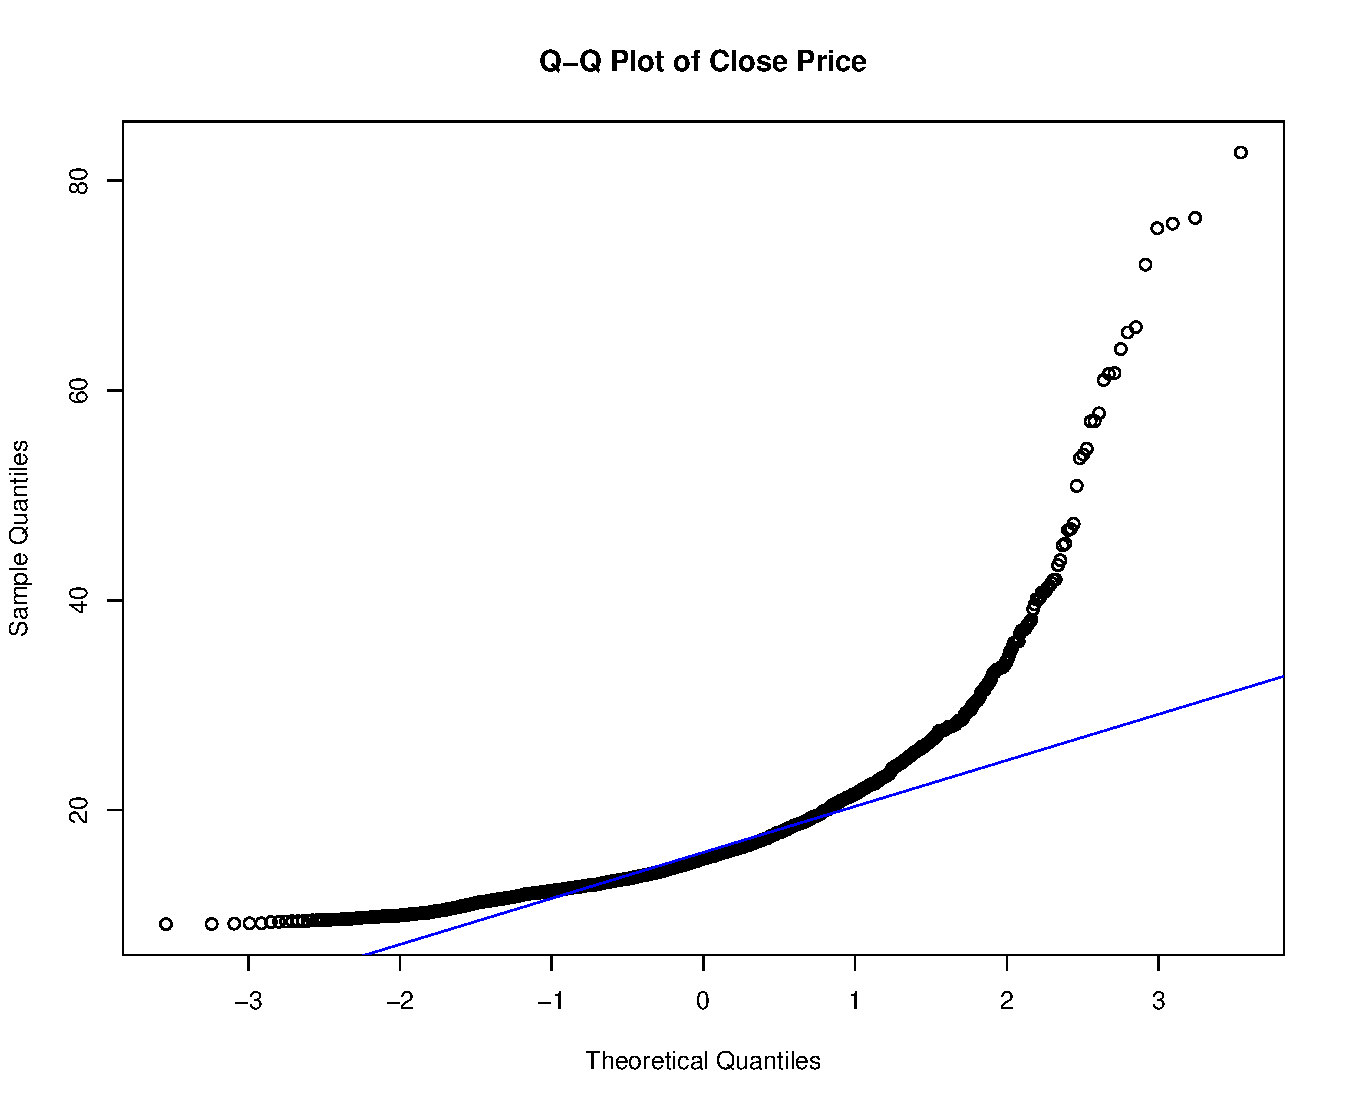
\includegraphics[width=\textwidth]{QQPlot.pdf}
    \caption{Close Price QQPlot}
    \label{fig:QQPlot}
\end{figure}

\vspace{0.5cm}

\begin{figure}[ht]
    \centering
    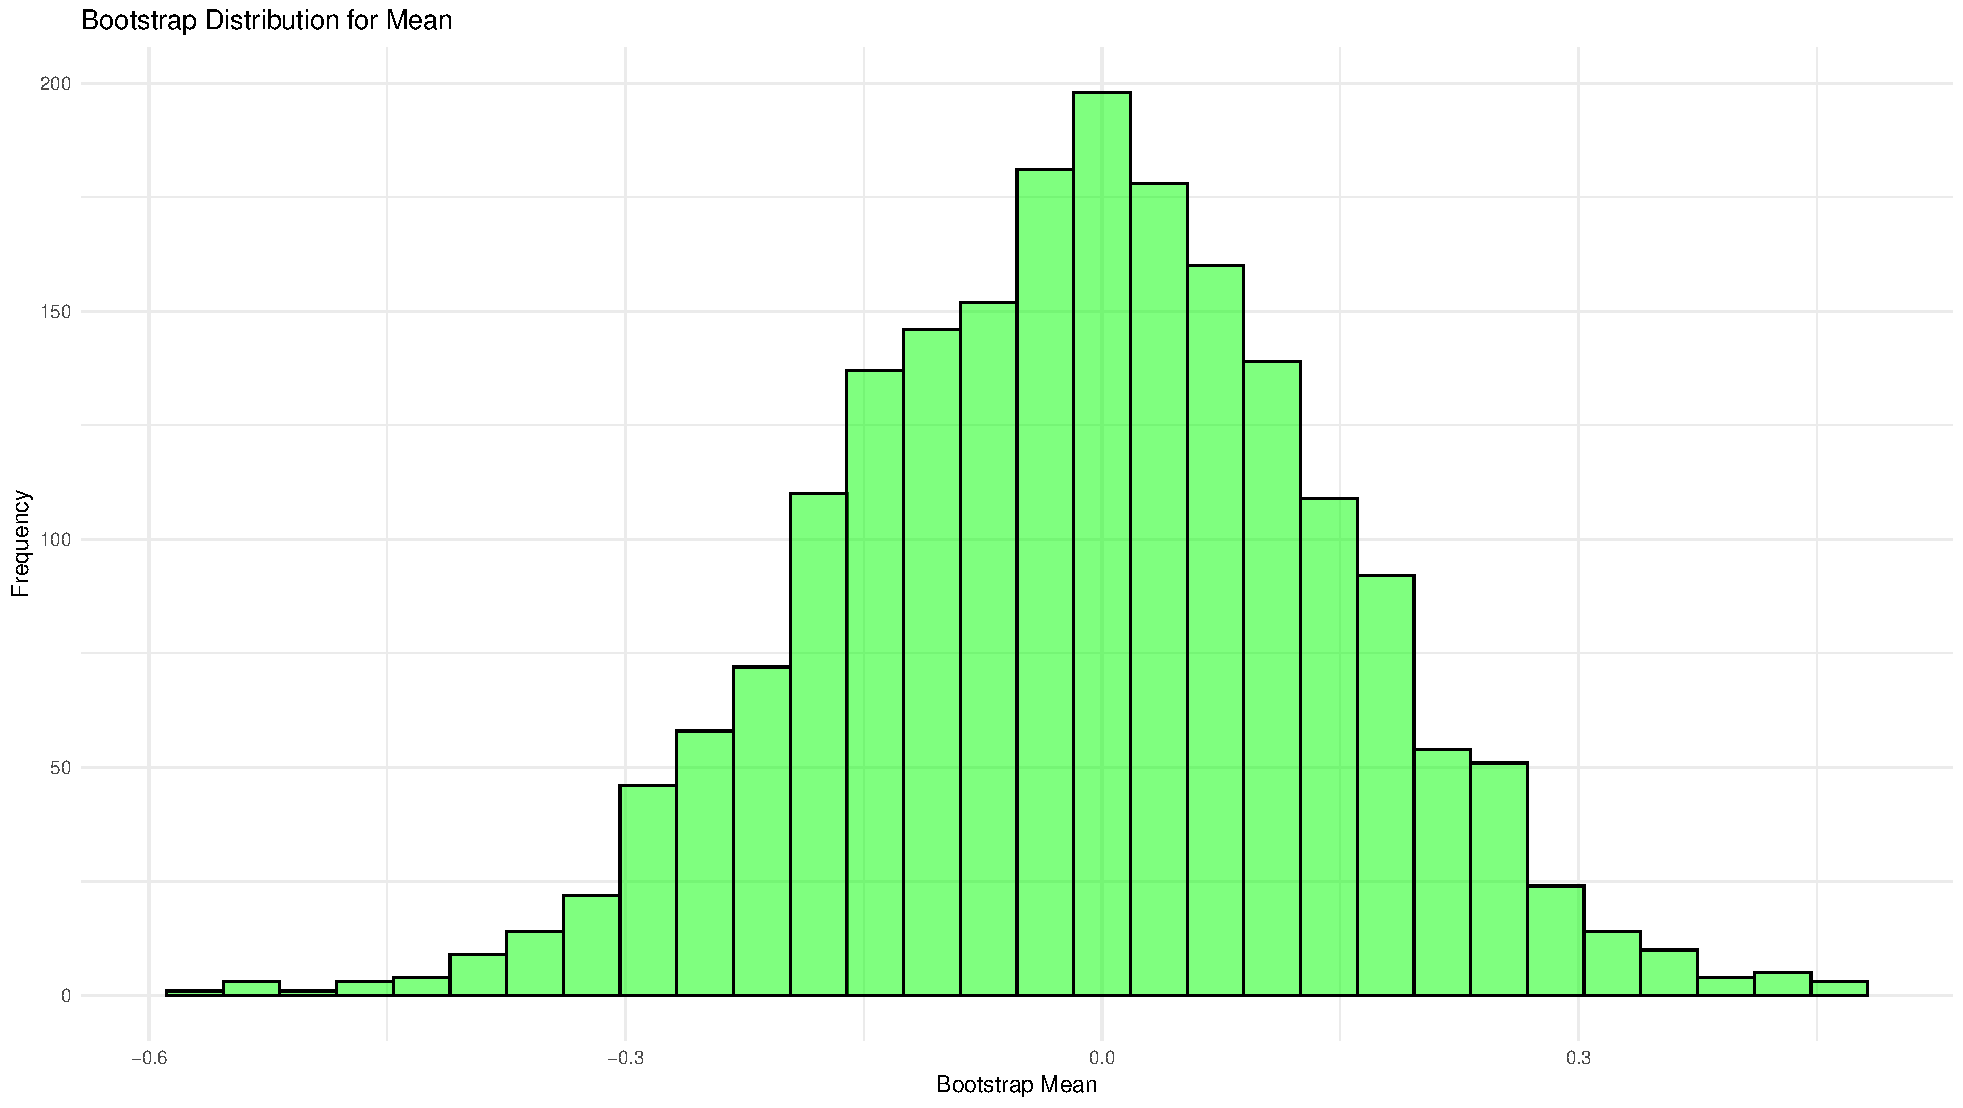
\includegraphics[width=0.9\textwidth]{MeanBS.pdf}
    \caption{Mean Bayesian Bootstrap Distribution}
    \label{fig:meanBS}
\end{figure}

\vspace{0.3cm}

\begin{figure}[ht]
    \centering
    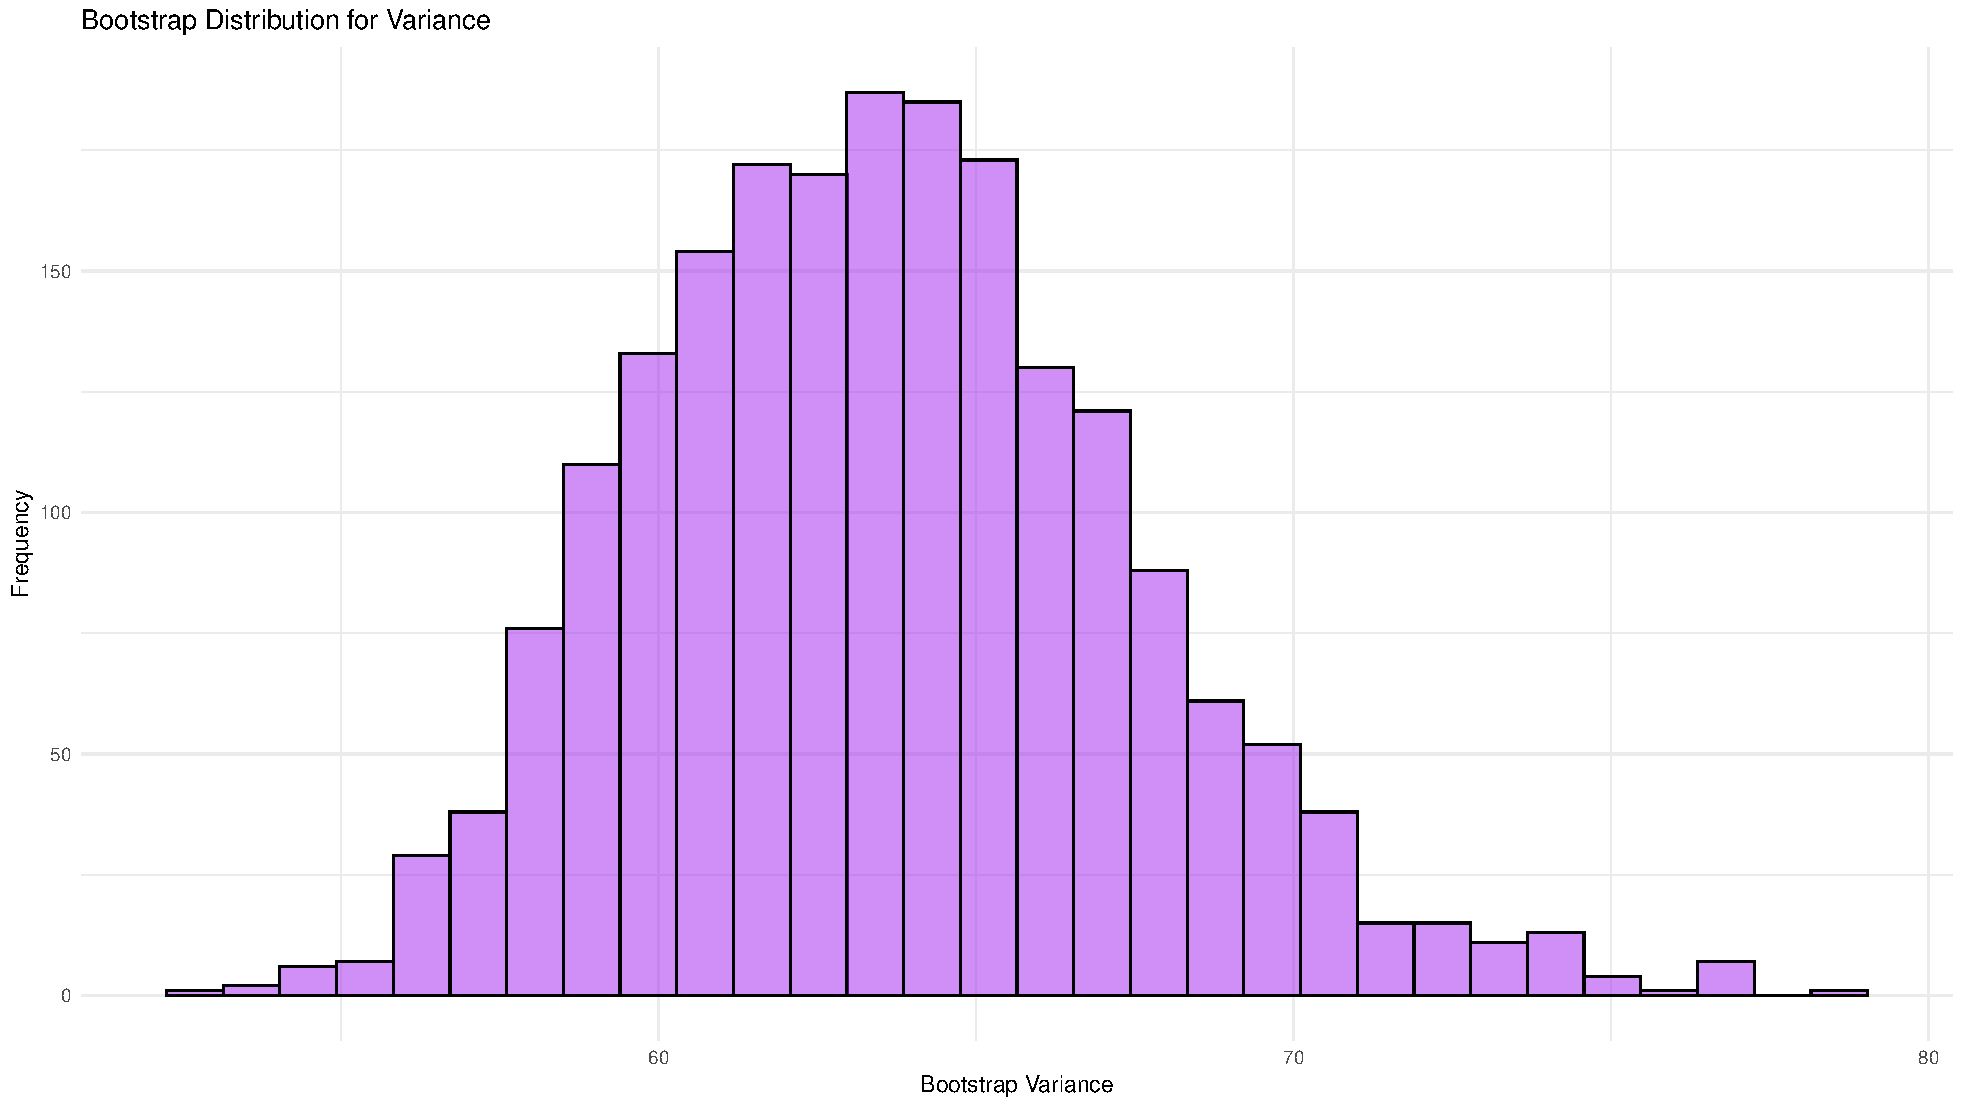
\includegraphics[width=\textwidth]{VarBS.pdf}
    \caption{Variance Bayesian Bootstrap Distribution}
    \label{fig:varBS}
\end{figure}

\begin{figure}[ht]
    \centering
    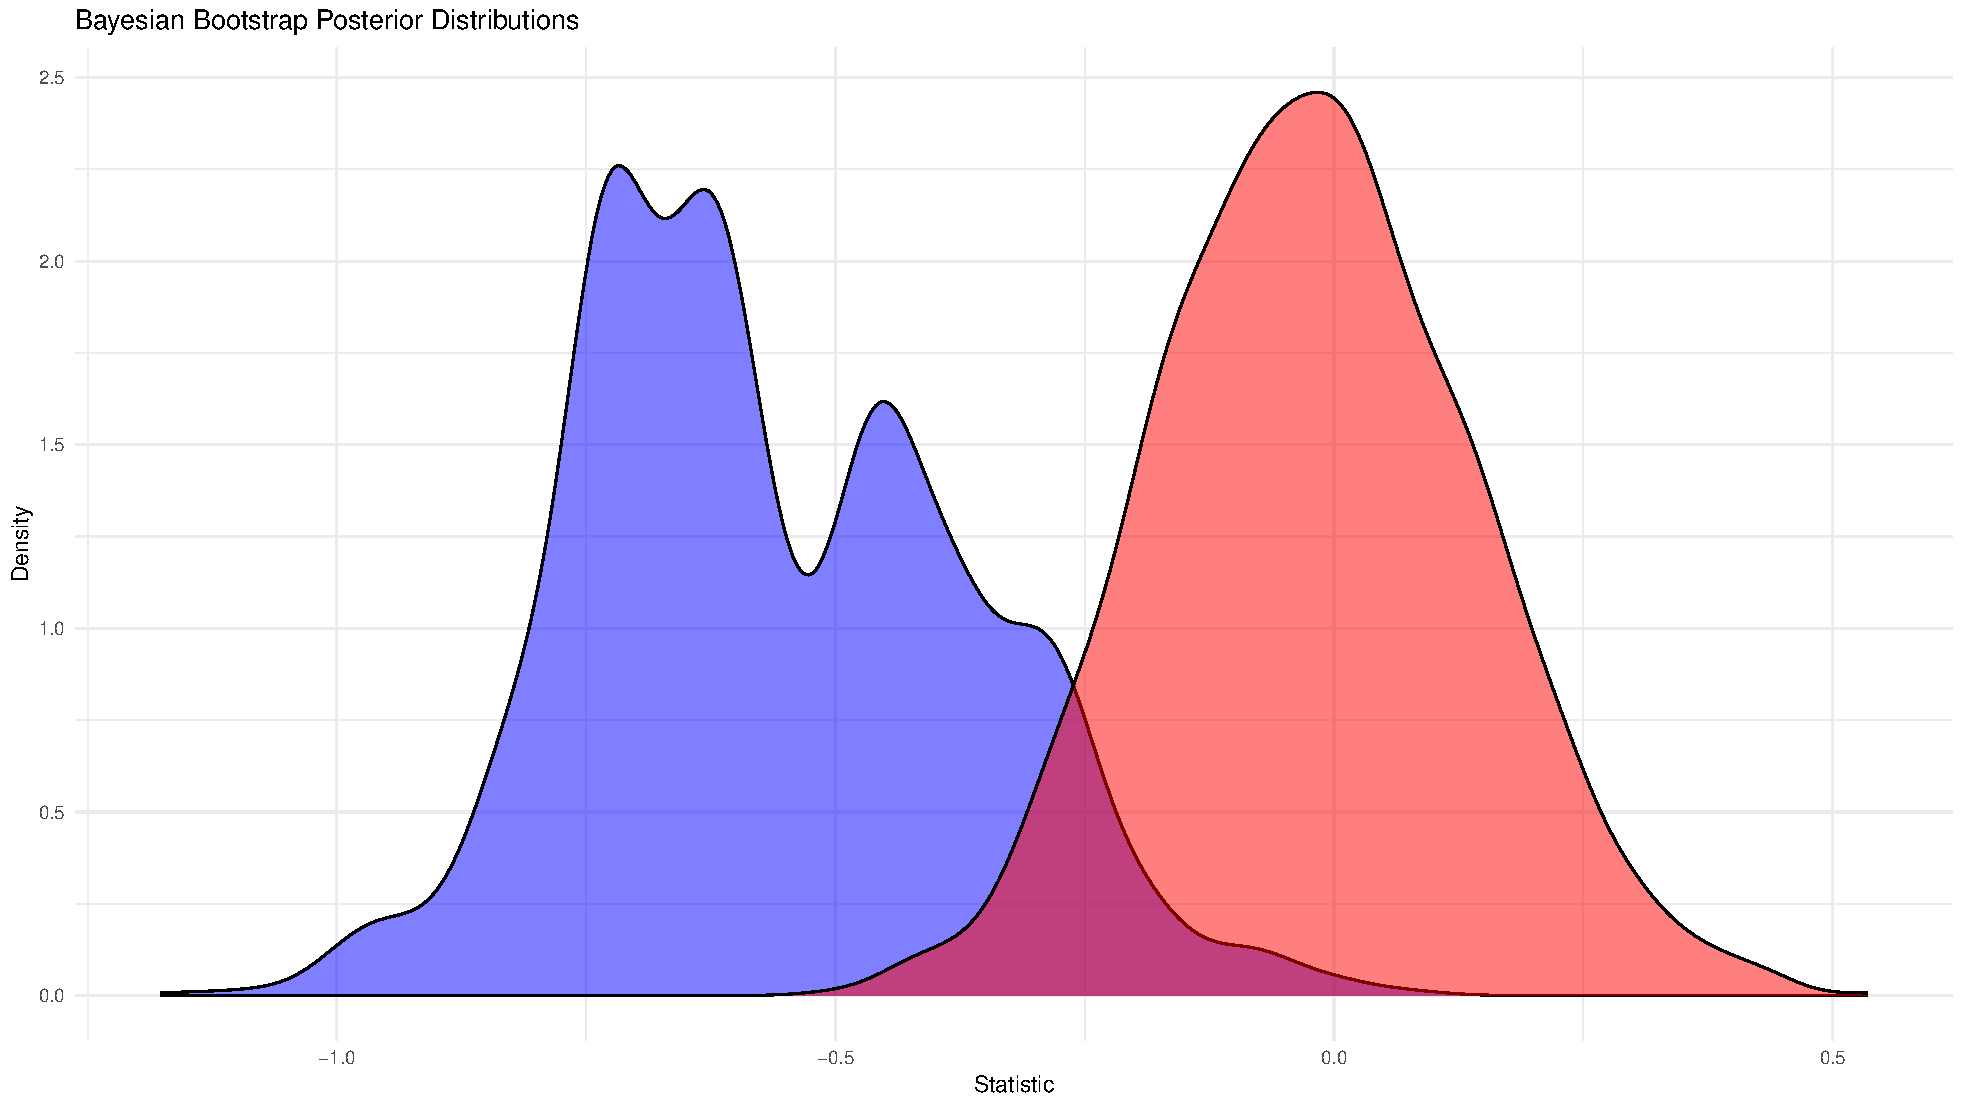
\includegraphics[width=\textwidth]{BayesBSPost.pdf}
    \caption{Bayesian Bootstrap Mean and Median Posterior Distributions}
    \label{fig:BayesBSPost}
\end{figure}

\begin{figure}[ht]
    \centering    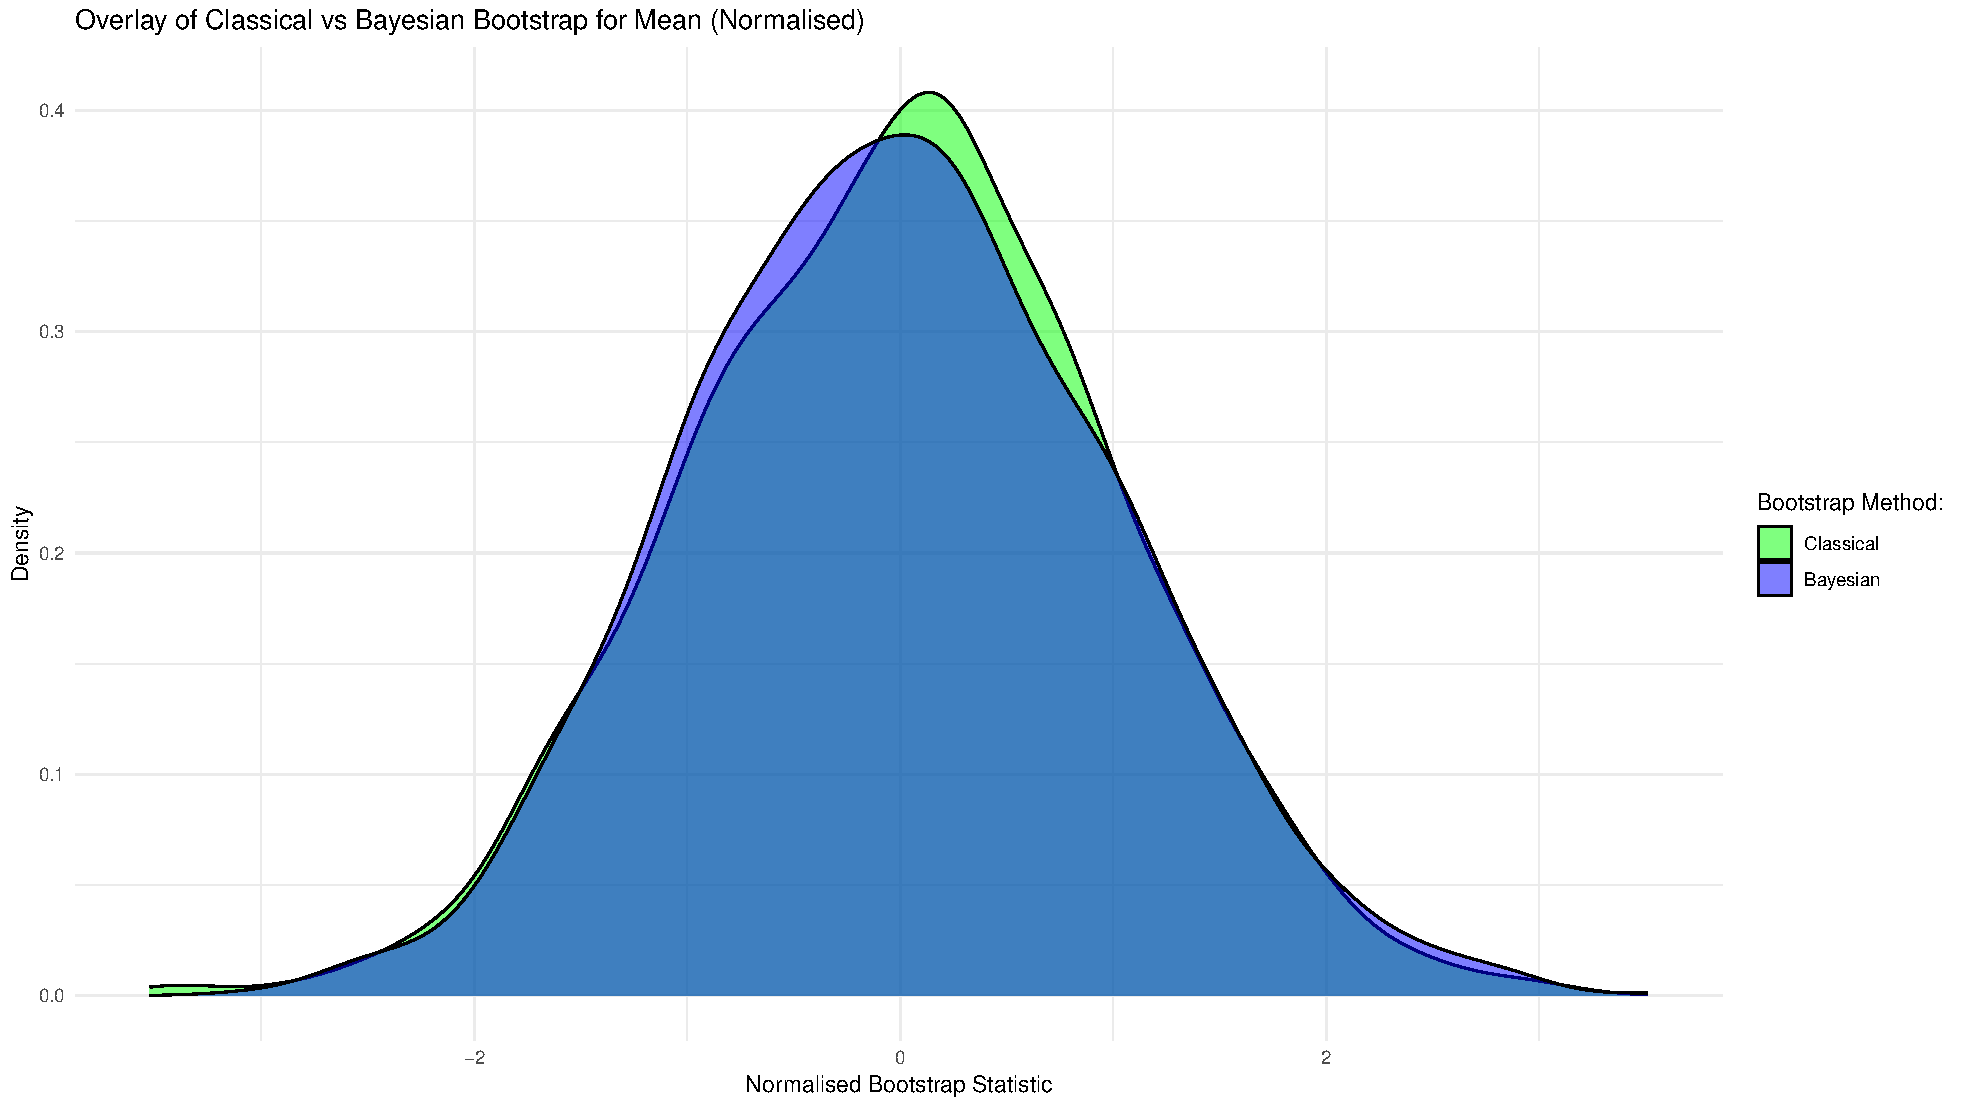
\includegraphics[width=\textwidth]{ClassBayesNorm.pdf}
    \caption{Classical and Bayesian Bootstrap Overlay}
    \label{fig:ClassBayesNorm}
\end{figure}

\vspace{0.3cm}

\begin{figure}[ht]
    \centering
    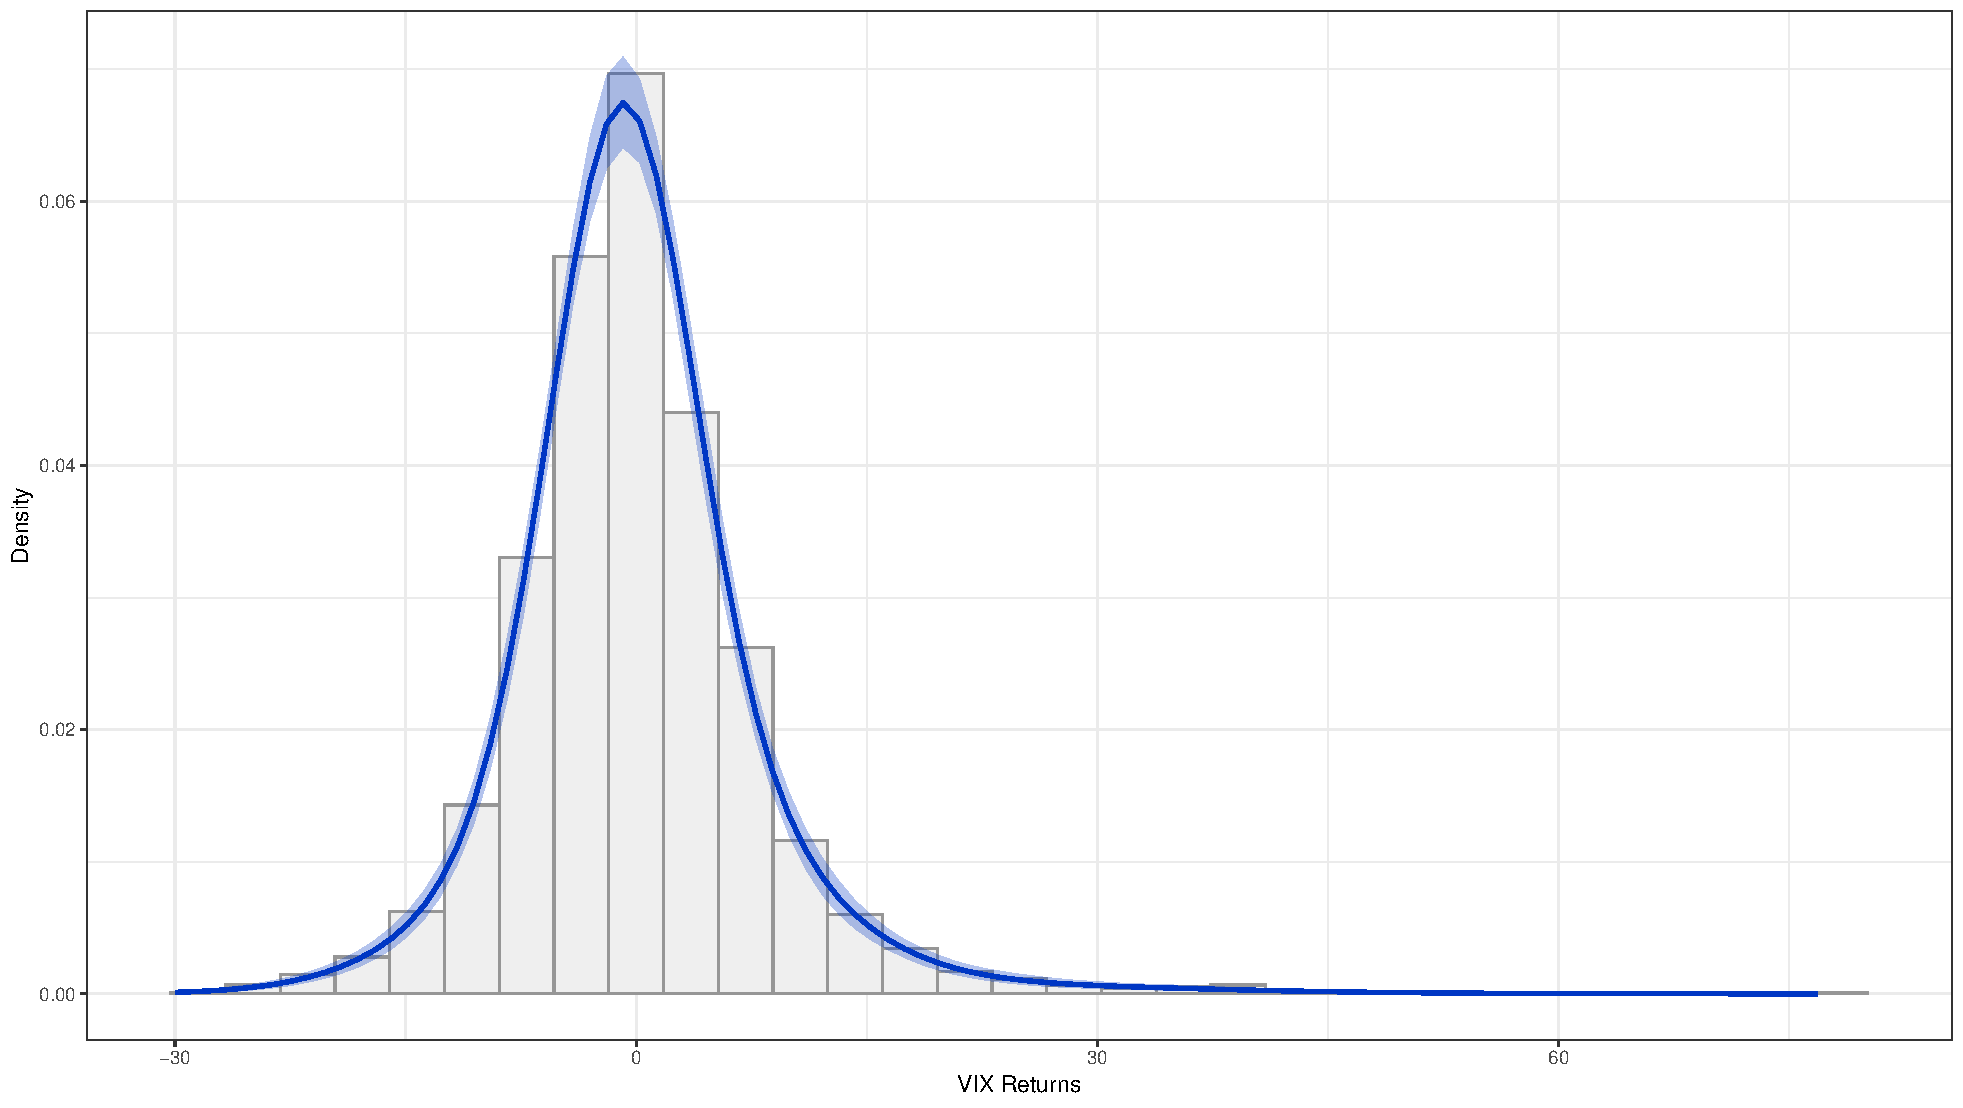
\includegraphics[width=\textwidth]{DPMMposteriordensity.pdf}
    \caption{DPMM Posterior Density}
    \label{fig:DPMMposteriordensity}
\end{figure}

% Full-width figures again
\begin{figure}[ht]
    \centering
    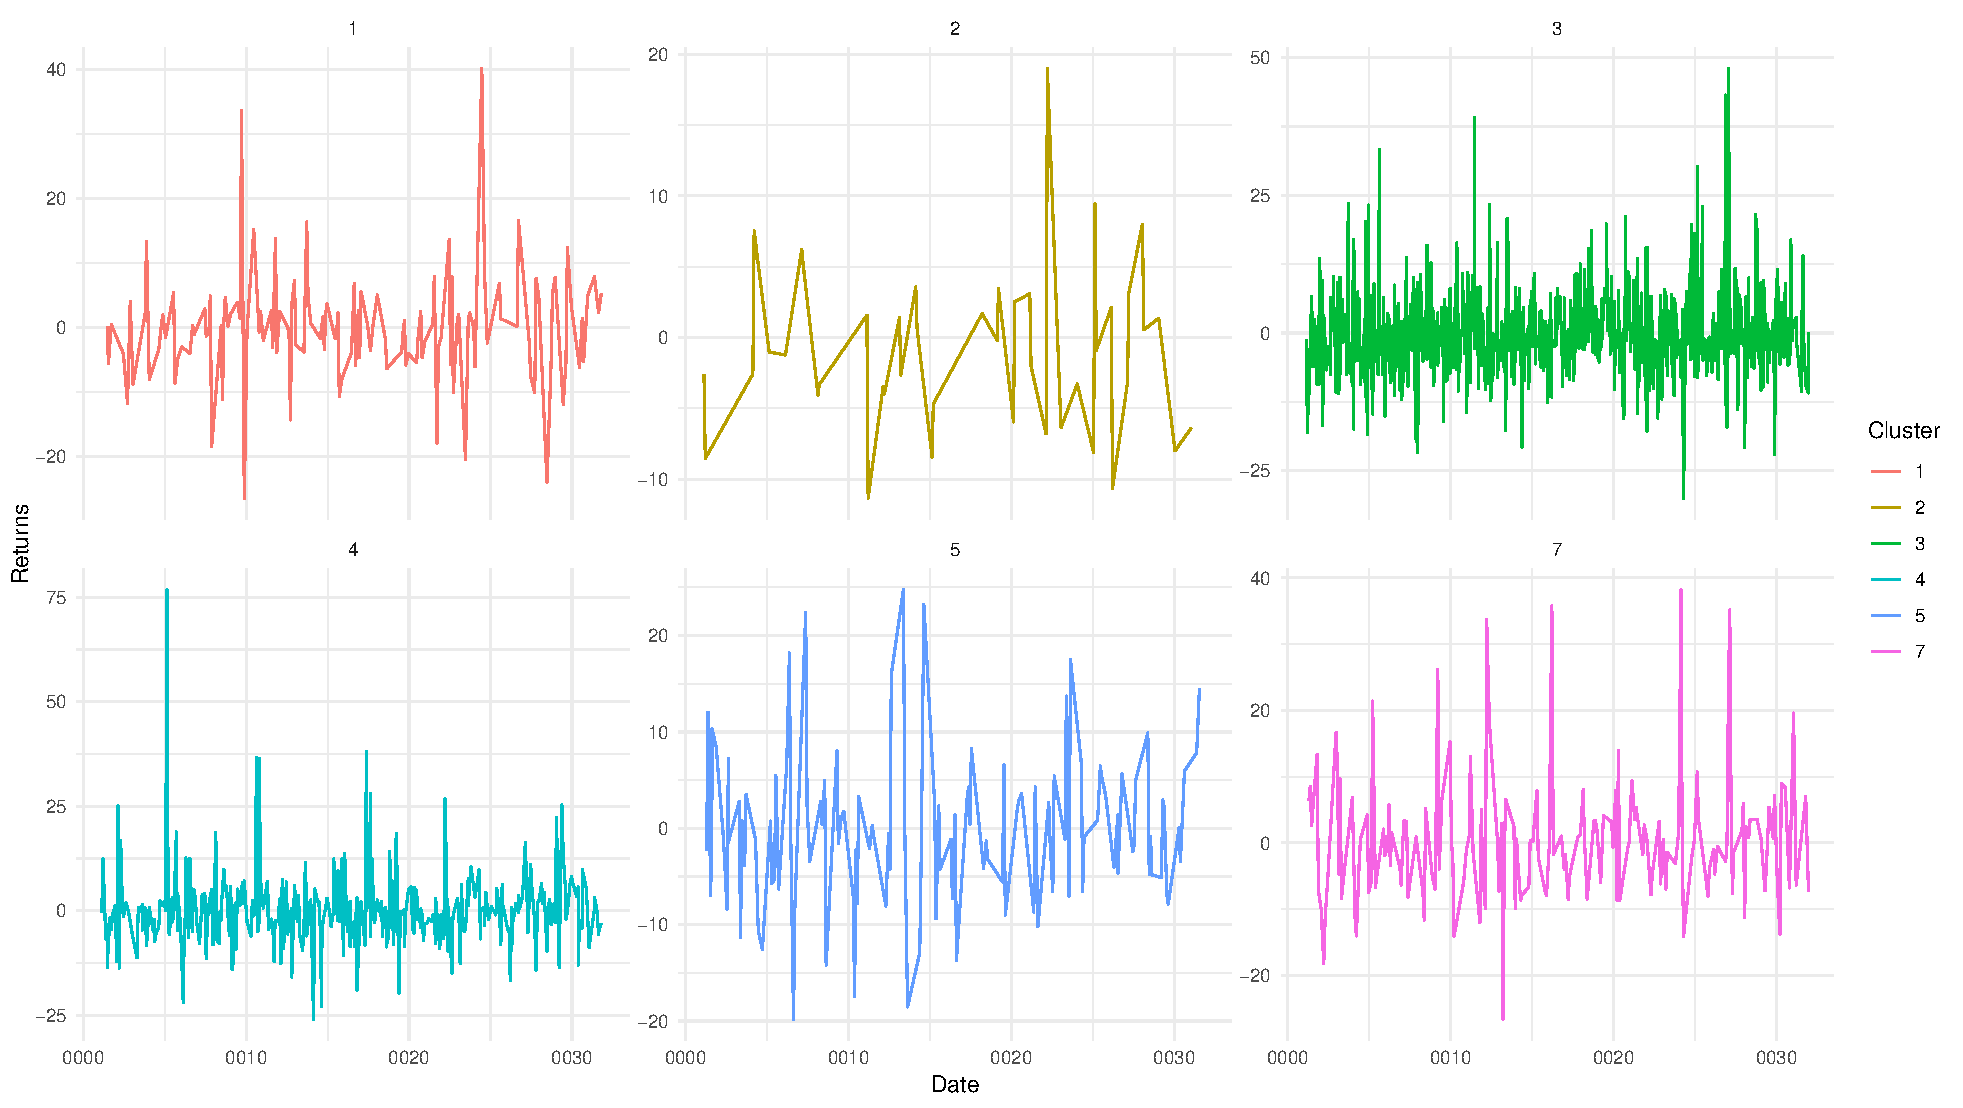
\includegraphics[width=\textwidth]{TimeClust.pdf}
    \caption{Time Series for common DPMM Clusters}
    \label{fig:TimeClust}
\end{figure}

\begin{figure}[ht]
    \centering
    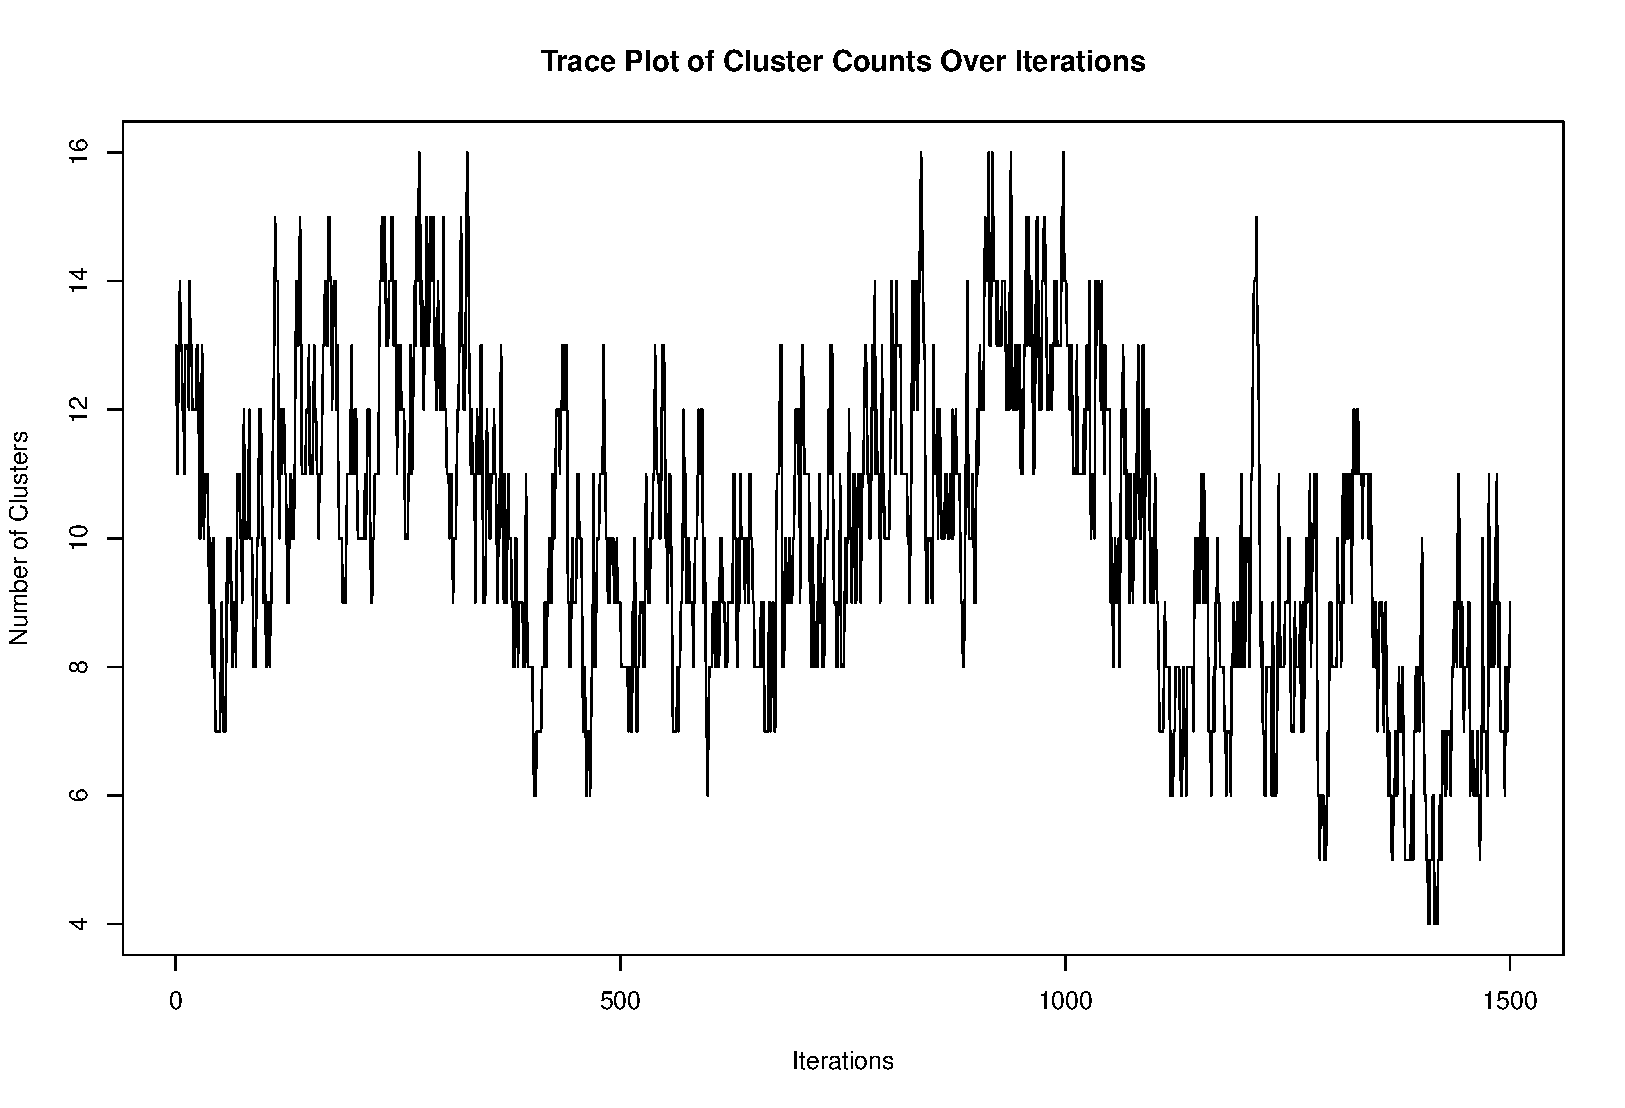
\includegraphics[width=\textwidth]{Trace Plot.pdf}
    \caption{Trace Plot of DPMM Cluster Counts Over Iterations}
    \label{fig:TracePlot}
\end{figure}

\end{document}

